\documentclass[11pt,a4paper,oneside]{article}
\usepackage[left=2cm, right=1.5cm, top=1.5cm]{geometry}
\usepackage{color}
\usepackage[utf8]{inputenc} % Включаем поддержку UTF8  
\usepackage[russian]{babel}  % Включаем пакет для поддержки русского языка  
\usepackage{graphicx}
\usepackage{enumitem}

\graphicspath{ {./images/} }
\DeclareGraphicsExtensions{.png,.pdf,.jpeg,.jpg}

\DeclareUnicodeCharacter{F7}{$\div$}
\DeclareUnicodeCharacter{3B1}{$\alpha$}
\DeclareUnicodeCharacter{3C0}{$\pi$}
\DeclareUnicodeCharacter{2190}{$\leftarrow$}
\DeclareUnicodeCharacter{2192}{$\rightarrow$}
\DeclareUnicodeCharacter{2191}{$\uparrow$}
\DeclareUnicodeCharacter{221A}{$\sqrt{}$}
\DeclareUnicodeCharacter{2260}{$\neq$}
\DeclareUnicodeCharacter{2A7E}{$\geq$}


\providecommand{\tightlist}{%
    \setlength{\itemsep}{0pt}\setlength{\parskip}{0pt}}

\title{Калькулятор}
\makeindex

\begin{document}
\maketitle
\tableofcontents
\pagebreak

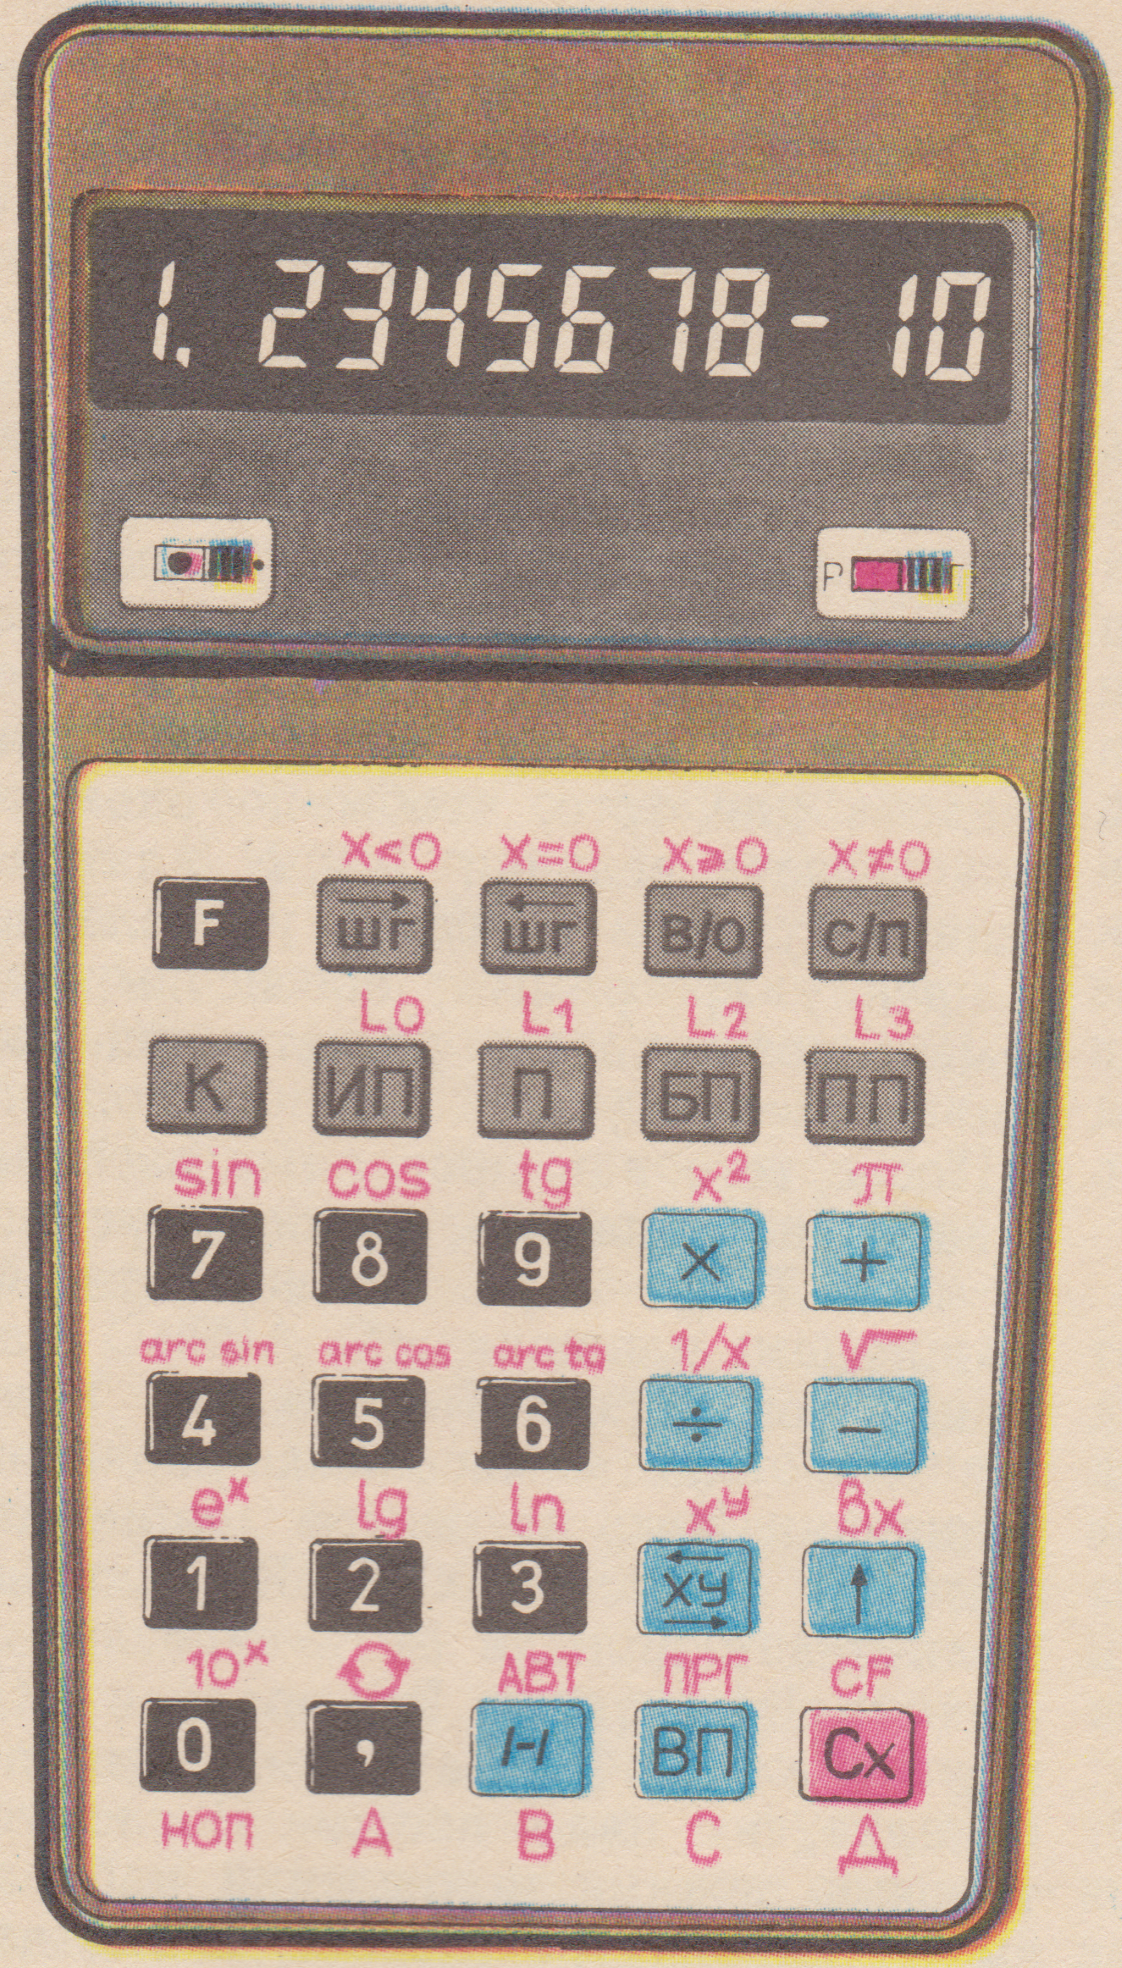
\includegraphics[width=6cm]{calculator}
\section{Логика микрокалькулятора}
ИГОРЬ ДАНИЛОВ, кандидат технических наук

Почему микрокалькулятор называется программируемым? Потому что в его память можно записать программу. Но как это сделать?

Режим ввода программы устанавливается клавишами «F ПРГ». Подобно тому как использование переключателя «Р—Г» не подразумевает совершения конкретных операций, клавиша «ПРГ» тоже лишь задает режим интерпретации вводимой информации. Режим же вычислений (не совсем удачно названный в "Руководстве по эксплуатации" автоматической работой) автоматически устанавливается при включении микрокалькулятора. А если нужно перейти к режиму вычислений после ввода программы, необходимо нажать клавиши «F АВТ».

Итак, включаем микрокалькулятор, нажимаем клавиши «F ПРГ». В правом углу экрана появляются цифры 00. Наш ПМК готов к приему программы.

Программа для ПМК представляет собой набор команд-инструкций, следуя которым машина обрабатывает информацию. Полная совокупность команд вместе с правилами их употребления и толкования образует язык микрокалькулятора. Как известно, учить иностранный язык лучше всего, разбирая написанные на нем несложные тексты. Вот и мы начнем с несложных программ — текстов на языке ПМК.

В предыдущей статье мы рассматривали решение простой физической задачи в режиме вычислений. Теперь для тех же целей напишем программу.

Напомним условие. Брусок массой m = 350 г скользит под действием силы, приложенной к нему под углом а. Ускорение бруска $а=0,3 m/c^{2}$, коэффициент трения $k=0,11$. Ускорение свободного падения принять равным $g=9,8 m/c^{2}$. Найти зависимость силы натяжения нити Т и давления бруска на поверхность N от угла а.

В общем виде решение записывается формулами:

x=cosa; y=sina; z=m/(x+ky);

T=z(a+kg); N=z(gx—ay), уже приведенными к виду, наиболее удобному для программирования.

\begin{tabular}{|c|c|c|c|c|c|}\hline
АДРЕС & КОМАНДА & КОД & АДРЕС & КОМАНДА & КОД \\\hline
00 & Fcos & 1Г & 16 & + & 10 \\\hline
01 & П1 & 41 & 17 & X & 12 \\\hline
02 & FBx & 0 & 18 & с/п & 50 \\\hline
03 & FSin & 1C & 19 & ИПД & БГ \\\hline
04 & П2 & 42 & 20 & ИП1 & Б1 \\\hline
05 & ИПВ & БL & 21 & X & 12 \\\hline
06 & X & 12 & 22 & ИПА & 6- \\\hline
07 & + & 10 & 23 & ИП2 & Б2 \\\hline
08 & ИПС & БС & 24 & X & 12 \\\hline
09 & Х4 & 14 & 25 & - & 11 \\\hline
10 & ÷ & 13 & 25 & ИП3 & БЗ \\\hline
11 & П3 & 43 & 27 & X & 12 \\\hline
12 & ИПВ & БL & 28 & с/п & 50 \\\hline
13 & ИПД & БГ & 29 & БП & 51 \\\hline
14 & X & 12 & 30 & 00 & 00 \\\hline
15 & ИПА & Б- & & & \\\hline
\end{tabular}

\begin{tabular}{|c|c|c|c|c|}\hline
КОМАНДА & \multicolumn{4}{|c|}{ИНДИКАТОР} \\\hline
Fcos & 1Г & & & 01 \\
П1 & 41 & 1Г & & 02 \\
FBX & 0 & 41 & 1Г & 03 \\
Fsin & 1С & 0 & 41 & 04 \\\hline
\end{tabular}

А это — программа. Она записана в трех колонках: первая — адрес команды, вторая — сама команда (клавиши, нажимаемые при вводе), третья — код команды. На втором рисунке в первой колонке — команда, во второй — содержимое экрана после ее ввода. Крайнее слева число — код последней введенной команды, затем коды двух предыдущих и, наконец, последняя пара цифр — адрес команды, которую надо вводить. Нам коды нужны для визуального контроля правильности ввода, для машины же они являются именами, названиями команд. Каждый код — двузначное число, правда, не в десятичной, а в шестнадцатеричной системе счисления. Хранится код каждой введенной команды в ячейке, адрес которой высвечивается на экране перед вводом этой команды.

Но как быть, если при вводе допущена ошибка? Если вы увидели, что код набранной команды не соответствует записанному в третьем столбце программы, то нажмите клавишу ← «ШГ» (шаг назад) и повторите ввод. Например, при вводе программы на экране светятся цифры: 1Г 0 41 04. Значит, при вводе команды по адресу 03 произошла ошибка: вместо синуса введен косинус. Нажимаем «ШГ», на экране: 0 41 1Г 03. Повторяем ввод команды «F sin». Читаем: 1C 0 41 04. Теперь все верно.

Но вот программа введена. Если сравнить ее с последовательностью нажатия клавиш для решения задачи из предыдущего выпуска, то легко убедиться, что программа почти полностью повторяет тот же набор. Те же символы знаков операций (сложение — команды по адресам 07 и 16, вычитание — по адресу 25, умножение — 06, 14, 17, 21 и 24), обращение к функциям (sin — адрес 03, cos — адрес 00), команда перемены местами содержимого регистров X и Y (адрес 09) и вызов содержимого регистра XI в регистр X (адрес 02). Но две команды нам еще не встречались. Это «С/П» (18 и 28) и «БП 00». Последняя команда в отличие от всех предыдущих размещается в двух смежных ячейках (по адресам 29 и 30).

Команда «С/П» (стоп/пуск) используется в программе для прекращения процесса вычислений, останова, как говорят программисты. В нашем случае остановки записаны после вычисления величин Т и N, чтобы можно было считать их значения с индикатора. В режиме вычислений эта команда останавливает либо запускает программу.

Команда "БП 00" (в общем случае — «БПnm», где nm — двузначное число от 00 до 97) читается так: безусловный переход на адрес 00. Она прерывает последовательное выполнение команд, записанных в программе. Следующей после этой команды выполняется та, что записана по адресу 00. У нас она введена для того, чтобы по окончании расчета величин Т и N для заданного угла α передать управление к началу программы, обеспечив тем самым возможность расчета при новом значении угла.

После того как программа введена и записана в память, нужно перевести наш ПМК в режим вычислений. Нажимаем клавиши «F АВТ». Машинка готова считать, но она пока что "не знает" числовых значений величин. На их месте записаны команды «ИП А», «ИП В» и т. д. Величина а должна быть записана в регистр RA, к - в RB, m — в RC, и g — в RД. Но сами они туда не попадут, их надо ввести. После установки режима вычислений набираем на клавиатуре нужное число, затем нажимаем клавиши «П» и номер регистра. Проведем эту работу: «0.3 ПА», «0.11 ПВ», «0.35 ПС», «9.8 ПД». Величины a, k, m и g записаны в соответствующие регистры. Теперь нужно сделать так, чтобы программа начала работать с того адреса, где записана ее первая команда (в нашем случае с нулевого). Нажимаем клавишу «В/О» (воз- врат/очистка). Наконец, нужно ввести переменную величину, значение угла α в градусах в регистр X (проверьте заодно, установлен ли переключатель «Р—Г» в положение «Г»), Набираем на клавиатуре нужное число, для начала 40. Нажим клавиши «С/П» запускает программу на счет. Примерно через 10 с на индикаторе появляется: 5.7639597—01. Первые 8 цифр — мантисса числа, две последние со знаком — порядок
числа. Снова нажимаем "с/п". Секунд через пять считываем второе число: 3.0594998. Если числа на экране другие, значит, при вводе программы допущена ошибка. Простейший путь исправить ее — выключить калькулятор, секунд через десять включить вновь и повторить ввод программы, строго контролируя каждый шаг.

Если же числа совпали, можно продолжать расчеты. Теперь достаточно набирать на клавиатуре значение угла в градусах и нажимать на клавишу «С/П». По результатам можно построить графики. Интересно, например, выяснить, при каком значении угла сила давления бруска на поверхность равна нулю. Правда, точное значение этого угла получить невозможно, зато его можно определить с большой степенью точности. Кстати, почему сила давления меняет знак? Что за смысл в отрицательном давлении? Чтобы ответить на этот вопрос, не обойтись без знания физики. Вот и пример использования ПМК при изучении этой науки.

Но вернемся к самому микрокалькулятору. Когда программа запущена, на экране мелькают цифры. Что происходит в это время внутри ПМК?

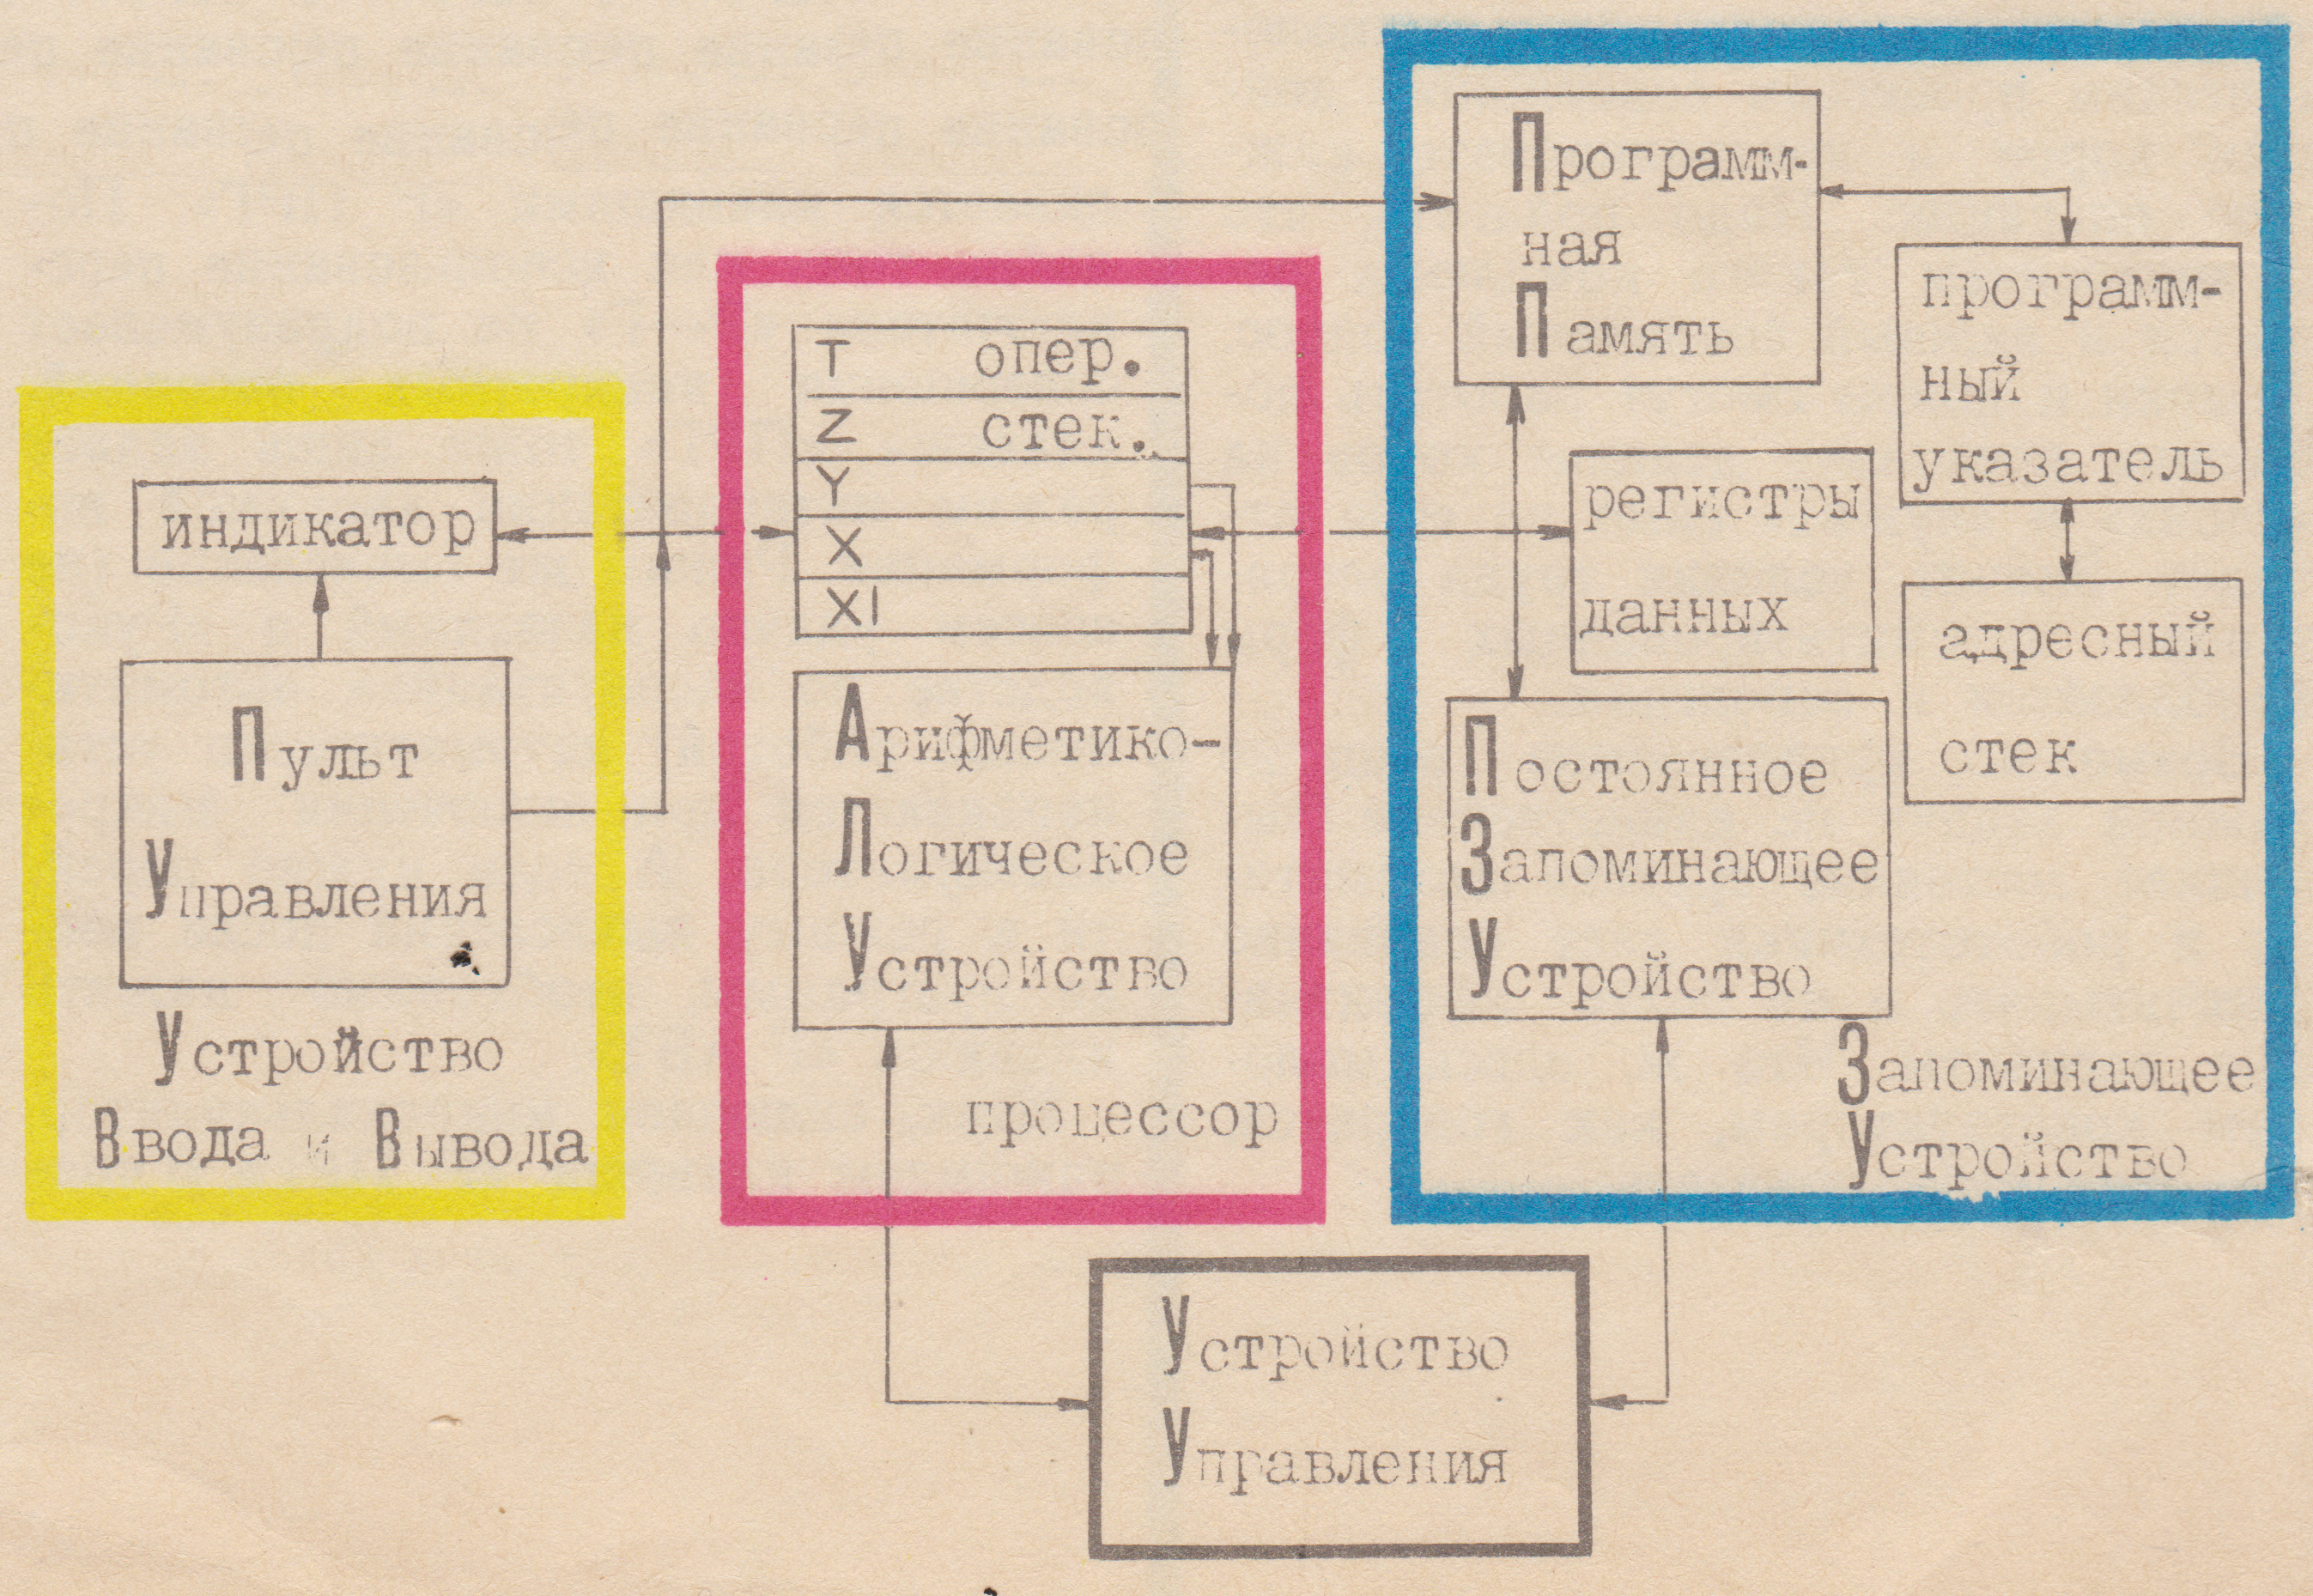
\includegraphics[width=\textwidth]{princip_scheme}

Принципиальная схема микрокалькулятора изображена на рисунке. Основными ее элементами являются устройство ввода и вывода информации (УВВ), устройство преобразования информации (процессор), запоминающее устройство (ЗУ) и устройство управления (УУ).

Устройство ввода и вывода — единственное, которое мы непосредственно видим. Состоит оно из клавиатуры, совмещающей функции устройства ввода и пульта управления, и индикатора. Программа и числа, вводимые с клавиатуры, отображаются на индикаторе. Туда же выводятся результаты вычислений. Индикатор, вообще говоря, — единственное "окно" в память машины, с помощью которого можно получить сведения о ее содержимом.

Команда, введенная с клавиатуры, попадает в запоминающее устройство. Состоит ЗУ из нескольких различных секций: программная память, регистры данных, постоянное запоминающее устройство (ПЗУ), а также программный указатель и адресный стек.

Программная память (ПП) представляет собой набор ячеек, в каждую из которых можно записать один код. Всего таких ячеек 98, нумеруются они двузначными числами  от 00 до 97. Количество ячеек определяет максимальную длину программы, которую можно ввести в память микрокалькулятору. Организована ПП наподобие "колеса обозрения". Адрес текущей ячейки записывается в программном указателе. При вводе команды адрес этот автоматически увеличивается на единицу и "колесо" поворачивается, подготавливая следующую "кабинку" (ячейку) для приема очередного "пассажира" (команды). Содержимое программного указателя можно изменять — с пульта или программным путем (об этом позже). При этом "колесо" может поворачиваться в любую сторону на заданное число позиций. Когда все 98 ячеек программной памяти заполнены, попытка ввести новую команду приводит к повороту "колеса" в начальное положение и команда попадает в первый адрес памяти, естественно стирая его старое содержимое.

Адресный стек состоит из пяти ячеек и используется для запоминания адреса команды, на которую нужно передать управление после окончания работы какой-либо подпрограммы (об использовании подпрограмм будет сказано в одной из следующих статей).

Регистры данных служат для записи и хранения числовой информации. Всего их 14. Таково максимальное количество чисел, которые можно одновременно хранить в памяти ПМК.

Постоянное запоминающее устройство содержит программы, которые, собственно, и организуют процесс вычислений. Эти программы нельзя изменить, они реализованы не программно, а аппаратно, то есть представляют собой совокупность электронных схем. Их нельзя даже прочесть, к ним можно лишь обращаться и получать результаты их работы. Именно программы из ПЗУ подсчитывают значения функций, названия которых записаны на клавиатуре, обеспечивают выполнение арифметических операций.

Выполняет же все операции по программам, хранящимся в ПЗУ, процессор — точнее, арифметическо- логическое устройство (АЛУ), работающее совместно с операционным стеком. В этом стеке 5 регистров: XI, X, Y, Z, Т. Числа движутся по регистрам либо автоматически (при выполнении некоторых операций), либо подчиняясь специальным командам. Подробно движение информации в стековых регистрах будет рассмотрено в одной из следующих статей. Особо важны два регистра: X и Y. Из них АЛУ черпает числовую информацию для выполнения двухместных операций: сложения, вычитания, умножения, деления и возведения в степень. Одноместные операции: извлечение квадратного корня, возведение в квадрат, вычисление тригонометрических функций и т. д. — производятся над содержимым регистра X.

В соответствии с кодом команды АЛУ вырабатывает результат операции и помещает его в регистр X. На экране отображается лишь содержимое этого регистра. Так что на индикаторе во время работы ПМК мелькают промежуточные результаты вычислений, появляющиеся в регистре X.

Наконец, устройство управления обеспечивает совместную работу всех блоков ПМК.

Зная функции отдельных элементов микрокалькулятора, проследим теперь полный цикл его работы при выполнении программы. Предположим, что она уже введена в память, установлен режим вычислений и все необходимые числа введены в нужные регистры. Нажимом клавиши «В/О» мы очищаем программный указатель, то есть устанавливаем его содержимое равным нулю. Клавиша, «С/П» запускает программу. Устройство управления считывает команду, адрес которой записан в программ ном указателе. После ее анализа и определения типа операции команда пересылается в АЛУ. По сигналам, поступившим из УУ, процессор вырабатывает результат операции. Затем УУ опрашивает программный указатель и выясняет, какая команда должна выполняться следующей. Потом цикл повторяется. Время выполнения цикла зависит от типа команды и колеблется от десятых долей секунды для команд типа записи и считывания, а также операций типа сложения, до нескольких секунд для вычисления тригонометрических функций. Знание времени выполнения отдельных команд помогает строить более быстродействующие программы.

Теперь подведем итоги.
\begin{enumerate}
\tightlist
\item Микрокалькулятор может работать в двух режимах: 1) ввода и редактирования программ и 2) вычислений. Первый устанавливается клавишами «F ПРГ», второй — «F АВТ». При включении ПМК автоматически устанавливается режим вычислений.
\item Программа для микрокалькулятора состоит из последовательности команд, вводится с клавиатуры и записывается в программную память. Помните, что адрес, который высвечивается при вводе в правом углу индикатора, — это адрес следующей вводимой команды.
\item Порядок работы с программой.
\begin{enumerate}[label=\arabic*)]
\item Установить режим «F ПРГ».
\item Ввести программу.
\item Перейти в режим вычислений «F АВТ».
\item Ввести постоянные в адресуемые регистры.
\item Установить начальный адрес считывания программы.
\item Набрать на клавиатуре значение переменного параметра.
\item Запустить программу на счет.
\item Если нужно повторить расчет для другого значения переменного параметра, перейти к пункту 6.
\end{enumerate}
\item Максимальная длина программы — 98 шагов, максимальное количество чисел, которые могут одновременно храниться в памяти, — 14.
\end{enumerate}

\subparagraph{двоичная система}
10 + 10 = 100!
Это не ошибка и не опечатка. Именно такой результат получается, если числа записаны в двоичной системе счисления.

Системой счисления называется способ выражения и записи чисел. Числа записываются в виде последовательности специальных символов. Смысл каждого символа зависит от позиции или разряда, в котором он записан. Количество единиц младшего разряда, объединяемого в одну единицу старшего, называется основанием системы, а символы, используемые для обозначения единиц каждого разряда, — цифрами.

Наиболее употребительна десятичная система. Мы настолько привыкли к этой системе, что "раскрываем" любое число не задумываясь. Например, $512 = 2 + 1 * 10 + 5*10^{2}$. Эта система представляется нам столь же естественной, как ребенку — родной язык. Но любая система счисления столь же естественна, как и любой язык. В вычислительной технике используются двоичная, восьмеричная и шестнадцатеричная система. Двоичная — самая простая и наиболее удобная для технической реализации. Цифр в ней всего две — 0 и 1. Когда в разряде (а называется двоичный разряд "бит"; несколько двоичных разрядов, чаще всего восемь, объединяются в "байт" — величину, с которой ЭВМ работает как с одним целым) накапливаются две единицы, то они заменяются единицей старшего разряда. Число $2_{10}$ (цифрой внизу обозначается основание системы) в двоичной системе записывается как $10_{2}$. Вообще любое число, записанное в n-ричной системе, переводится в десятичную очень просто. К последней n-ричной цифре прибавляется предпоследняя, умноженная на n, затем стоящая перед ней и умноженная на $n^{2}$, и т. д. Скажем, двоичное число $101_{2} = 1+0*2 + 1*2^{2} = 5_{10}$. Привлекательность двоичной системы, как уже говорилось, — в простоте технической реализации. Каждый разряд — это некоторое устройство, которое может находиться всего в двух состояниях.

В микрокалькуляторе для размещения одного символа кода отводится "тетрада" — четыре двоичных разряда. Легко подсчитать максимальное число, которое можно записать таким образом: $1111_{2} = 1 + 1 * 2 + 1 * 2^{2} + 1 * 2^{3} = 15_{10}$. Значит, коды должны изображаться числами в шестнадцатеричной системе. Так как десятичных знаков для изображения таких чисел не хватает, приходится "выдумывать" дополнительные символы. В ПМК число 10 изображается символом «—», 11 — «L», 12 — «С», 13 — «Г», 14 — «Е». "Цифра" 15 в обозначениях кодов не используется.

\section{Язык микрокалькулятора}
ИГОРЬ ДАНИЛОВ,
кандидат технических наук

Язык микрокалькулятора (как и любой язык) представляет собой набор символов, а также правил, определяющих, как с помощью этих символов писать и понимать написанное.

Правда, в отличие, скажем, от русского языка, где слова расчленяются на буквы, изменяются при склонении или спряжении, язык микрокалькулятора напоминает скорее китайский либо японский. Его "словарь" состоит из несклоняемых слов-иероглифов, и лишь порядком их следования определяется смысл текстов — программ для ПМК. Каждый из иероглифов — это имя команды: надпись на клавише или над ней (а в нижнем ряду — и под клавишей). Клавиши К и F самостоятельной роли не играют: по своему действию они подобны переключателю регистров пишущей машинки. Если требуется иероглиф, начертанный на клавише, то нужно нажать только ее, если же иероглиф, написанный над клавишей, то предварительно необходимо воспользоваться клавишей F (а в некоторых случаях — клавишей К). Каждая команда, независимо от количества нажимаемых клавиш (а оно для некоторых команд доходит до трех), отображается в памяти и на индикаторе одним двузначным шестнадцатеричным числом — кодом. Исключение составляют команды переходов: после них указывается адрес перехода, поэтому за кодом команды обязательно следует код этого адреса.

Полный набор команд «Электроники БЗ-34» приведен в таблице. Ею могут пользоваться и владельцы микрокалькуляторов «Электроника МК-54» и «Электроника МК-56» — система команд у них та же самая. Различаются лишь некоторые обозначения X → П вместо П, П→X вместо ИП, X ←→У вместо XY и В↑ вместо ↑, а также названия обратных тригонометрических функций — $sin^{-1}$, $cos^{-1}$, $tg^{-1}$ вместо arcsin, arccos, arctg. Смысл же операций и их коды полностью идентичные приведенным в таблице.

Условно всю совокупность команд можно разбить на два класса. К первому относятся команды, используемые в программе; ко второму — команды, предписывающие порядок работы ПМК. Последние вводятся в режиме вычислений; мы рассмотрим их при описании процесса отладки программ.

Первый класс можно подразделить на четыре группы: 1) вычислительные команды; 2) команды обмена информацией; 3) команды управления ходом вычислений; 4) команды, использующие режим косвенной адресации. Последние по своим функциям не отличаются от команд второй и третьей групп, но, поскольку используют иной режим адресации, будут рассмотрены отдельно. Особняком стоит команда К НОП.

К первой группе относятся прежде всего команды арифметических операций: сложение + (код 10), вычитание — (11), умножение X (12) и деление ÷(13). Все они двухместные — работают с содержимым двух регистров стека X и Y, причем при вычитании в X записывается вычитаемое, а при делении — делитель. Результат каждой из арифметических операций заносится в регистр X, прежнее содержимое этого регистра перемещается в XI. То, что было в Y, пропадает, замещаясь числом из регистра Z, а в Z заносится содержимое регистра Т. Но при этом прежнее содержимое регистра Т остается и на своем месте.

Надо сказать, что микрокалькулятор способен работать не со всякими числами. Максимальное не должно превосходить $10^{100}$ (точнее, $9,9999999*10^{99}$), минимальное должно быть не меньше $10^{99}$ — в противном случае вместо нормального восьмиразрядного числа в память и на индикатор запишется "чистый" нуль. Наибольшую осторожность надо соблюдать при умножениях и делениях. Иногда случается, что конечный результат цепочки операций лежит в пределах возможностей ПМК, а на промежуточном этапе возникает аварийная остановка. Её можно избежать, правильно организуя процесс вычислений.

Рассмотрим простой пример. Нужно вычислить значение дроби $a*b/c$, где $а=2*10^{51}$, $b=3*10^{49}$, $с=4*10^{50}$. Легко видеть, что результат ($1,5*10^{50}$) лежит в допустимых пределах. Но если соответствующий фрагмент программы записать так: ИП А, ИП В, X, ИП С, ÷, то есть сначала выполнять умножение (мы считаем, что исходные величины хранятся в одноименных регистрах), то после первого же действия получается число $6*10^{100}$, возникает "аварийный" останов, на экране появляется сообщение ЕГГО.Г и вычисления прекращаются. Если же выполнять сначала деление (например, записать тот же фрагмент так: ИП А, ИП С, ÷, ИП В, X)» то никаких неприятностей не произойдет.

К арифметическим можно отнести и команду (—) (код 0L). Она одноместная, использует только регистр X. При ее выполнении меняется знак числа, находящегося в этом регистре (плюс на минус или наоборот).

Остальные вычислительные команды используются для расчета значений различных функций. Их названия написаны над соответствующими клавишами. Чтобы получить значение какой-либо из них, нужно предварительно нажать клавишу F, но для краткости при описании команд мы ее упоминать не будем.

Какие же функции доступны нашему ПМК? Вот они: извлечение квадратного корня $\sqrt{}$ (код 21);
возведение в квадрат $X^{2}$ (22); получение обратной величины $1/X$ (23); возведение числа 10 в любую степень $10^{x}$ (15) и возведение в степень числа е, основания натуральных логарифмов $e^{x}$ (16); вычисление десятичного и натурального логарифмов lg (17) и ln (18); вычисление тригонометрических функций (аргументы могут быть заданы как в градусах, так и в радианах) sin (1C), cos (1Г), tg (1E), а также обратных тригонометрических функций arcsin (19), arccos (1—) и arctg (1L). Аргумент для каждой из этих функций берется из регистра X, туда же записывается результат, а аргумент после выполнения операции перемещается в XI. Содержимое других регистров не меняется.

Особняком среди команд подобного рода стоит $Х^{y}$ (24) — возведение произвольного числа в любую степень. Возводимое число берется из регистра X, а показатель степени — из Y. После выполнения команды результат, как и обычно, заносится в X, то, что было там прежде, переходит в XI, а вот содержимое Y, как и остальных регистров, остается на месте. Отметим, что эту команду «Электроника БЗ-34» выполняет хуже других: результата приходится ждать долго, да и точность его ниже, чем при выполнении других команд. Так, $2^{2}$, вычисленное по этой команде, "равно" 3,9999996. А вот если использовать команду $X^{2}$, результат равен в точности четырем. Калькуляторы же первых выпусков при выполнении команды $X^{y}$ иногда вообще ошибаются. Так что рекомендуем по возможности ее избегать.

Вычислительные команды способны работать не со всеми возможными числами. Иногда это ограничения чисто математические (нельзя, скажем, извлекать квадратный корень из отрицательного числа или вычислять его логарифм), иногда диктуются возможностями ПМК. Поскольку числа, доступные микрокалькулятору, ограничены по абсолютной величине, то аргументы функций $10^{x}$ и $e^{x}$ не могут превосходить соответственно 99,999999 и 230,25. Не допускаются и отрицательные аргументы, по абсолютной величине превосходящие эти числа. Функция $X^{y}$, независимо от величины показателя, не определена для отрицательных оснований. При вычислении тригонометрических функций запрещается выбирать в качестве аргумента числа, превышающие $10^{1}$ (независимо от того, измеряются ли они в градусах или в радианах).

Напомним, что в микрокалькуляторах типа «Электроника БЗ-34» используется обратная бесскобочная (или польская) запись арифметических выражений. Сначала выписываются аргументы операции, а потом ее символ — например, не аХb, а аbХ; не $\sqrt{c}$, а $c\sqrt{}$.

При составлении программ нужно следить, чтобы перед совершением каждой арифметической операции стек был заполнен так, как требуется для ее выполнения.

\begin{figure}[h]
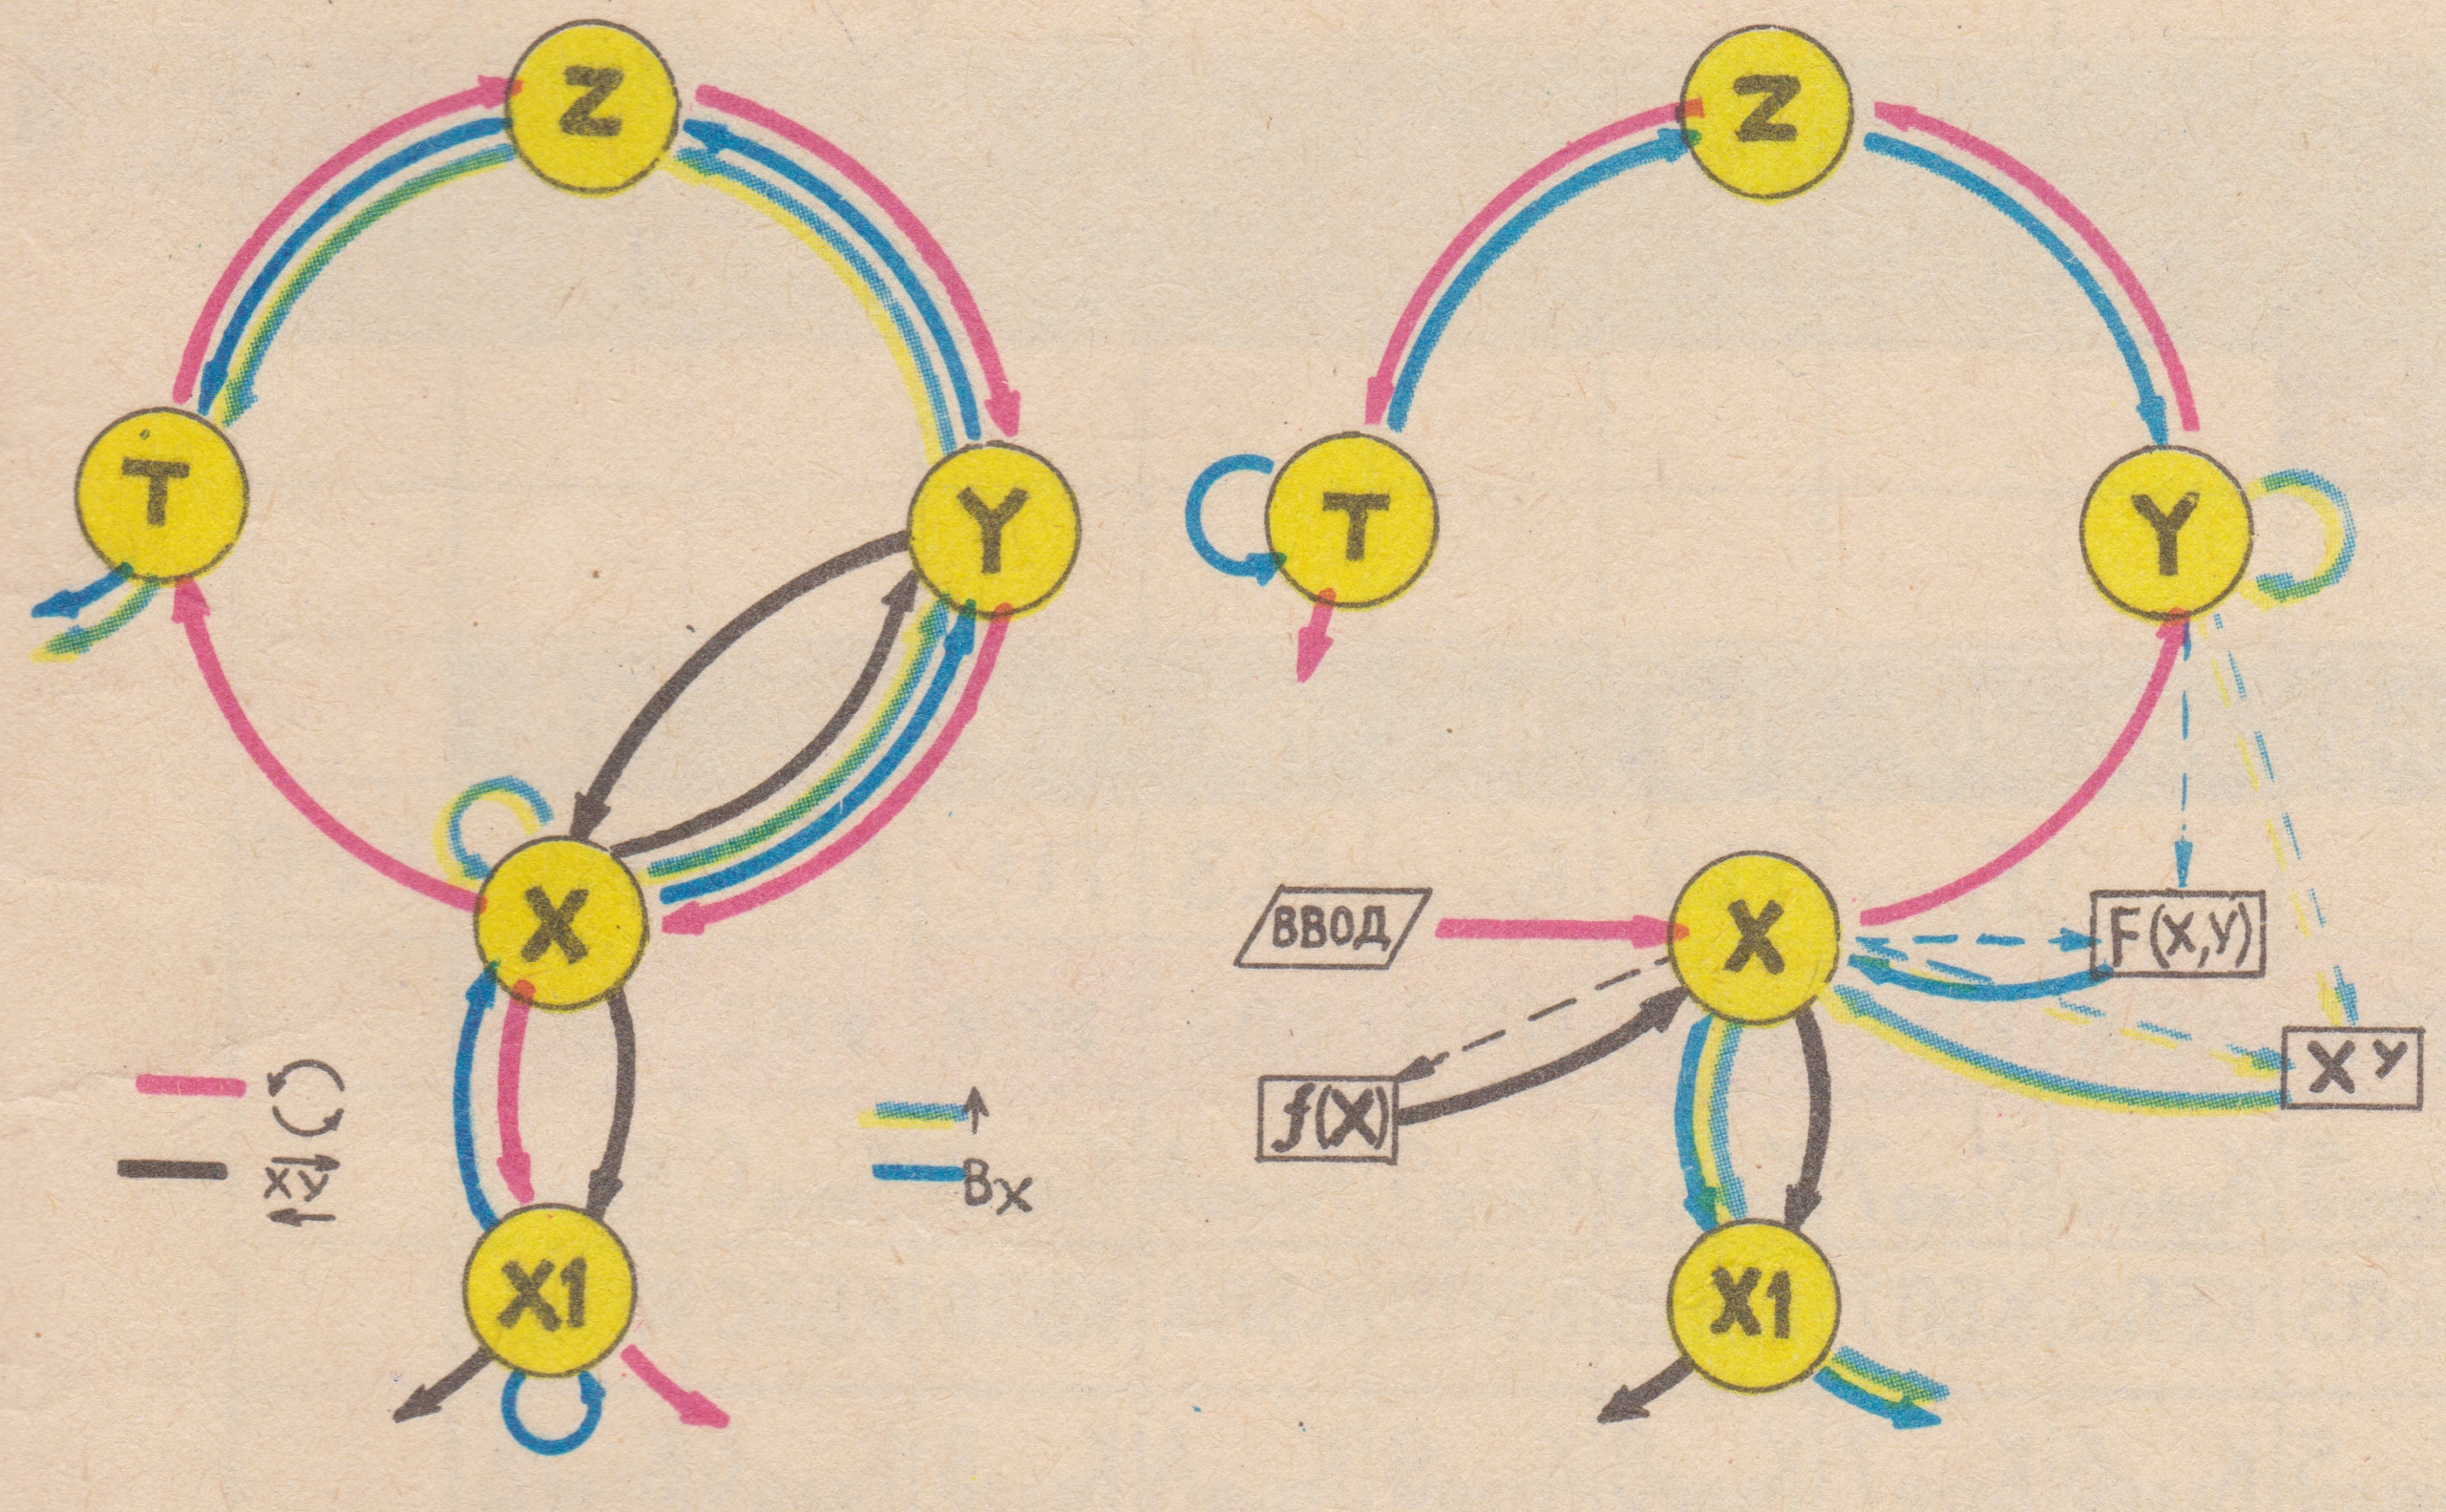
\includegraphics[width=\textwidth]{stack}
\caption{Движение информации по регистрам стена при выполнении команд обмена информацией (слева), ввода и вычислительных операции (справа).}
\end{figure}

Перемещением чисел по регистрам стека и по регистрам данных "заведуют" команды второй группы (команды обмена информацией). Это ↑(ОЕ), F Вх (0), XY (14) и FO (25). Первая из них, ↑ используется чаще всего для разделения вводимых чисел. Она сдвигает числа в стеке "снизу вверх" (см. рис.), сохраняя содержимое регистра X и выбрасывая за пределы стека число, хранившееся в регистре Т. F Bx используется для вызова содержимого регистра предыдущего результата (XI) в регистр X. В остальном ее действие подобно действию предыдущей команды; сдвиг чисел в стеке "снизу вверх" и вытеснение содержимого регистра Т. Команда XY меняет местами содержимое регистров X и Y; при этом число, находившееся в регистре X, дополнительно копируется и в регистре XI, вытесняя его прежнее содержимое. То, что было в остальных регистрах, при этом не меняется. FO совершает круговой обмен: число из регистра X перемещается в Т, содержимое Y передвигается в X, Z — в Y, а Т — в Z. Пропадает при этом только содержимое регистра XI: туда копируется число из X. Движение информации при выполнении всех этих команд отражено на диаграммах.

Есть 14 команд, позволяющих пересылать содержимое регистра X в адресуемые регистры (или регистры данных). Всего их тоже 14. Первые десять обозначаются цифрами от 0 до 9, последние — буквами А, В, С, Д. Для занесения в них информации служат команды: ПО (код 40), П1 (41)... П9 (49). ПА (4—), ПВ (4L), ПС (4С) и ПД (4Г). Каждая из команд требует набора двух клавиш: П и номера регистра (цифры или буквы), но, как мы видим, отображаются они одним кодом — как в памяти, так и на индикаторе. Обратите внимание, что буквы А, В, С и Д написаны под клавишами, но после нажатия клавиши П воспринимаются именно они.

Для вызова информации из адресуемых регистров в регистр X служат команды ИП0 (код 60)... ИП9 (69), ИП А (6—)... ИП Д (6Г). Условно к ним можно отнести и команду Fπ, действие которой заключается в вызове записанного в ПЗУ числа π в регистр X.

В языке микрокалькулятора нет специальных команд ввода. Числа просто набираются на клавиатуре и автоматически заносятся в регистр X. Однако можно хранить числа и в программной памяти. Например, если нужно умножить содержимое регистра 0 на 2, мы пишем обычно: ИП0, 2, X. Теперь при работе программы число 2 вводить не надо — оно занесено в программную память, занимая в ней одну ячейку. Для многозначных чисел такая запись, как правило, нецелесообразна. Например, если мы решим занести в программную память вместо двойки число 2,58, то соответствующий фрагмент программы будет выглядеть так: ИП0, 2, «,», 5, 8, X. Одно число занимает целых четыре ячейки — слишком много! Однако если все адресуемые регистры заняты, а в ПП место есть, то волей-неволей приходится прибегать и к этому способу. Коды цифр совпадают с ними самими (от 00 до 09); кроме них, при вводе чисел в ПП используются символы «,» (код 0—) и ВП (ОС) — ввод порядка. Так, для записи в ПП числа $1,6*10^{-19}$ (заряд электрона в кулонах) нужно ввести команды: 1, «,», 6, ВП, 1, 9, /—/.

Последняя команда этой группы — Сх (код 0Г). Она "стирает" содержимое регистра X (вернее, засылает туда число 0).

Рассмотренных команд достаточно для написания несложных программ, производящих вычисления по последовательным формулам. Однако для многих задач этого набора недостаточно. Даже при решении элементарного квадратного уравнения требуется сначала проверить знак дискриминанта квадратного трехчлена, чтобы знать, вычислять ли действительные корни уравнения, или же действительную и мнимую части корней комплексных. То есть нужно сначала выбрать путь и лишь потом начинать вычисления.

В языке микрокалькулятора имеются средства для проведения подобных операций. Это команды управления программой.

Наиболее часто употребляется команда останова С/П (код 50). Она используется для приостановки процесса вычислений, когда нужно либо прочесть полученный результат, либо ввести с клавиатуры какие-нибудь числа или предписывающие команды. В каждой программе обязательно есть хотя бы одна команда С/П — не может же программа работать бесконечно!

Команда безусловного перехода БП (51) передает управление команде, адрес которой записан сразу после нее. Фактически она занимает в памяти две смежные ячейки: в первой записан код 51, во второй — другое двузначное число, адрес перехода. Так что две цифры подряд,набранные после команды БП, записываются одним кодом — числом от 00 до 97 (напомним, что память ПМК состоит из 98 ячеек, поэтому адресов 98 и 99 попросту нет).

Команды условного перехода тоже передают управление, но лишь при выполнении определенных условий. В качестве условия в этих командах нашего ПМК используется сравнение содержимого регистра X с нулем. Если условие, записанное в команде, выполнено, то управление передается на следующую по порядку команду, в противном случае — по указанному адресу. Например, условный переход х<0, 23 выполняется так. Если число, находящееся в регистре X, меньше нуля, то выполняется команда, следующая за приведенным фрагментом, в противном случае — команда, код которой записан по адресу 23. Команд условного перехода четыре: х<0 (5С), х=0 (5Е), х≠0 (57), х⩾0(59).
Поскольку названия их написаны над клавишами, то перед ними нужно нажимать клавишу F.

Есть среди команд перехода четыре команды, предназначенные для организации циклов — многократного выполнения заданной последовательности команд. Это L0 (код 5Г), L1 (5L), L2 (58) и L3 (5—). Перед каждой из них тоже, естественно, нажимается клавиша F. А после каждой указывается адрес перехода. При обращении к одной из команд организации цикла из содержимого соответствующего (имеющего тот же номер) регистра данных вычитается единица, и, если результат не равен нулю, управление передается по указанному адресу перехода. Если же результат равен нулю, цикл завершается, и выполняется команда, записанная после адреса перехода. Таким образом, заслав в один из первых четырех регистров данных некоторое число n, мы получаем возможность выполнить некоторую часть программы n раз.

Последняя из программ перехода — это ПП (код 53) — переход на подпрограмму. Структура ее такая же, как и у остальных: сначала записывается сама команда, за ней — адрес перехода. Но в отличие от команды БП она не только "безусловно" передает управление по заданному адресу, но и после отработки подпрограммы — а последнюю обязательно завершает команда В/О (возврат/очистка, код 52), — автоматически возвращает программу "на старое место" — к команде, следующей за ПП.

Особняком стоит команда К НОП (код 54), которая набирается двумя клавишами К и НОП. Это — "пустая" команда, она не совершает никаких действий. Употребляется обычно при отладке программ: если выяснится, что одна из команд лишняя, то, чтобы не переписывать остальные, на ее место записывают "пустую" команду.

Команды косвенной адресации мы рассмотрим позже. Подведем краткие итоги.

\begin{enumerate}
\item Язык микрокалькулятора — это набор команд, имена которых написаны на клавиатуре. Чтобы использовать команды, названия которых даны над клавишами, нужно предварительно нажать клавишу F. Перед командой НОП нужно нажать клавишу К.
\item Каждая вычислительная команда размещается в одной ячейке памяти.
\item Результаты работы вычислительных команд помещаются в регистр X. Исходные данные для одноместных операций черпаются из этого же регистра, а для двухместных — из регистров X и Y.
\item Во всех операциях по записи информации в регистры данных и по ее извлечению обязательно участвует регистр X. В регистры данных можно засылать только его содержимое, и только в него можно считывать числа из этих регистров.
\item Команды перехода записываются в двух смежных ячейках памяти (в первой — сама команда, во второй — адрес перехода). Адрес перехода обязательно набирается в виде двузначного, числа.
\item При использовании вычислительных команд нужно следить за тем, верно ли расположены в регистрах, стека аргументы операций, и, кроме того, помнить об ограничениях, накладываемых на величину аргументов. Если последняя выходит за пределы допустимых ограничений, работа программы прекращается и на индикатор выводится сообщение ЕГГОГ.
\item Старайтесь по возможности избегать употребления команды $X^{y}$. Работает она медленно, а ошибки при вычислениях дает большие.
\end{enumerate}

\section{Блок-схема - портрет программы}

\begin{table}[]
\begin{tabular}{|l|l|l|l|l|l|l|l|l|l|l|l|l|l|l|l|}
\rotatebox{90}{АДРЕС} & \rotatebox{90}{КОМАНДА} & \rotatebox{90}{код} & стек   &     &     &   &    & \rotatebox{90}{АДРЕС} & \rotatebox{90}{команда}                                                      & \rotatebox{90}{код} & стек                                                          &     &    &   &        \\
      &         &     & X      & У   & z   & т & XI &       &                                                              &     & X                                                             & y   & Z  & т & X1     \\
00    & ПА      & 4-  & a      &     &     &   &    & 31    & ИПА                                                          & 6-  & а                                                             & B   & d  &   &        \\
01    & с/п     & 50  & b      & а   &     &   &    & 32    & ÷                                                            & 13  & B/a                                                           & d   & а  &   &        \\
02    & ↑       & 0Е  & b      & b   & а   &   &    & 33    & /-/                                                          & OL  & Хr                                                            & d   & а  &   &        \\
03    & с/п     & 50  & c      & b   & а   &   &    & 34    & П1                                                           & 41  & Хr                                                            & d   & а  &   &        \\
04    & /-/     & OL  & -с=с1  & b   & а   &   &    & 35    & XY                                                           & 14  & d                                                             & Хr  &    &   &        \\
05    & ИПА     & 6-  & а      & с1  & b   &   &    & 36    & Fx\textless{}0 & 5C  &                                                               &     &    &   &        \\
06    & Fx=0    & 5Е  &        &     &     &   &    & 37    & 48                                                           & 48  &                                                               &     &    &   &        \\
07    & 23      & 23  &        &     &     &   &    & 38    & /-/                                                          & 0L  & -d                                                            & Хr  & а  &   &        \\
08    & FO      & 25  & с1     & b   & а   &   &    & 39    & F√ & 21  & √-d  & Xr  & а  &   & \\
09    & XY      & 14  & b      & с1  &     &   &    & 40    & ИПА                                                          & 6-  & а                                                             & √-d & Хг &   &        \\
10    & Fx≠o    & 57  &        &     &     &   &    & 41    & ÷                                                            & 13  & (√-d)/a                                                       & Ха  &    &   &        \\
11    & 19      & 19  &        &     &     &   &    & 42    & ИП5                                                          & 65  & г.                                                            & Xim & Хг &   &        \\
12    & ÷       & 13  & c1/b   &     &     &   &    & 43    & с/п                                                          & 50  &                                                               &     &    &   &        \\
13    & ипз     & 63  & Е01    & х1  &     &   &    & 44    & FO                                                           & 25  & Xim                                                           & Хr  &    &   &        \\
14    & с/п     & 50  &        &     &     &   &    & 45    & с/п                                                          & 50  &                                                               &     &    &   &        \\
15    & XY      & 14  & х1     & E01 &     &   &    & 46    & БП                                                           & 51  &                                                               &     &    &   &        \\
16    & с/п     & 50  &        &     &     &   &    & 47    & 59                                                           & 59  &                                                               &     &    &   &        \\
17    & БП      & 51  &        &     &     &   &    & 48    & F√                                                           & 21  & √d                                                            & Хr  & а  &   &        \\
18    & 59      & 59  &        &     &     &   &    & 49    & ИПА                                                          & 6-  & а                                                             & √d  & Хг &   &        \\
19    & ИП0     & 60  & Е00    & b   &     &   &    & 50    & ÷                                                            & 13  & (√d)/a                                                        & хr  &    &   &        \\
20    & с/п     & 50  &        &     &     &   &    & 51    & +                                                            & 10  & Xr+(√d)/a                                                     &     &    &   &        \\
21    & БП      & 51  &        &     &     &   &    & 52    & ИП1                                                          & 61  & Хr                                                            & X1  &    &   & (√d)/а \\
22    & 59      & 59  &        &     &     &   &    & 53    & FBx                                                          & 0   & (√d)/a                                                        & Хr  & X1 &   &        \\
23    & X       & 12  & ас1    & b   & а   &   &    & 54    & -                                                            & 11  & Xr-(√d)/a &     &    &   &        \\
24    & XY      & 14  & b      & ас1 & а   &   &    & 55    & ИП4                                                          & 64  & Е02                                                           & Х2  & X1 &   &        \\
25    & 2       & 02  & 2      & b   & ас1 & а &    & 56    & с/п                                                          & 50  &                                                               &     &    &   &        \\
26    & ÷       & 13  & b/2=B  & ас1 & а   &   &    & 57    & FO                                                           & 25  & х2                                                            & X1  &    &   &        \\
27    & пв      & 4L  & B      & ас1 & а   &   &    & 58    & с/п                                                          & 50  &                                                               &     &    &   &        \\
28    & Fx2     & 22  & B2     & ас1 & а   &   &    & 59    & БП                                                           & 51  &                                                               &     &    &   &        \\
29    & +       & 10  & B2+ac1 & а   &     &   &    & 60    & 00                                                           & 00  &                                                               &     &    &   &        \\
30    & ипв     & 6L  & B      & d   & а   &   &    &       &                                                              &     &                                                               &     &    &   &       
\end{tabular}
\end{table}


\end{document}
